\section{Metodyka Scrum} \label{scrum}

Jednym z~podstawowych celów niniejszej pracy inżynierskiej jest przedstawienie wykorzystanych w~niej technologii, narzędzi i~metod.


\textit{Scrum} \cite{scrumaliance} (z~ang. przepychanka, młyn) jest jedną z~wielu pochodnych metodyki programowania zwinnego \cite{agile1} (ang. \textit{agile programming}).

\subsection{Programowanie zwinne} \label{scrum.agile}

\textit{Programowanie zwinne} jest popularną metodą pracy w~wielu firmach parających się programowaniem. Dla wyjaśnienia, czym tak naprawdę jest, wystarczy definicja \cite{agile2}:

\begin{quote}
,,\textit{Programowanie zwinne} (ang. \textit{agile software development}) to~grupa metodyk wytwarzania oprogramowania opartego o~programowanie iteracyjne (model przyrostowy). Wymagania oraz~roz\-wią\-za\-nia e\-wo\-lu\-ują przy współpracy samozarządzalnych zespołów, których celem jest przeprowadzanie procesów wytwarzania oprogramowania. Pojęcie zwinnego programowania zostało zaproponowane w 2001 w~\textit{Agile Manifesto} \cite{agile.manifesto}
[\ldots]


Generalnie metodyka oparta jest o~zdyscyplinowane zarządzanie projektem, które zakłada częste inspekcje wymagań i rozwiązań wraz z~procesami adaptacji (zarówno specyfikacji jak i~oprogramowania). Metodyka ta~najczęściej znajduje zastosowanie w~małych zespołach programistycznych, w~których nie występuje problem komunikacji, przez co~nie trzeba tworzyć rozbudowanej dokumentacji kodu. Kolejne etapy wytwarzania oprogramowania zamknięte są~w~iteracjach, w~których za~każdym razem przeprowadza się testowanie wytworzonego kodu, zebranie wymagań, planowanie rozwiązań itd. Metoda nastawiona jest na~szybkie wytwarzanie oprogramowania wysokiej jakości.''
\end{quote}

\subsection{Scrum} \label{scrum.scrum}

Poniżej omówiono metodykę \textit{Scrum}, wykorzystaną podczas realizacji części praktycznej pracy. Metodyka \textit{Scrum} opiera się na~ścisłych iteracjach, w~których realizowane są~założenia projektowe. Każda iteracja zaczyna się tzw. \textit{Sprint~Meeting'iem} (z~ang. ,,spotkanie w~biegu'') \cite{scrumaliance}.

\begin{figure}[!t]
\centering
\fbox{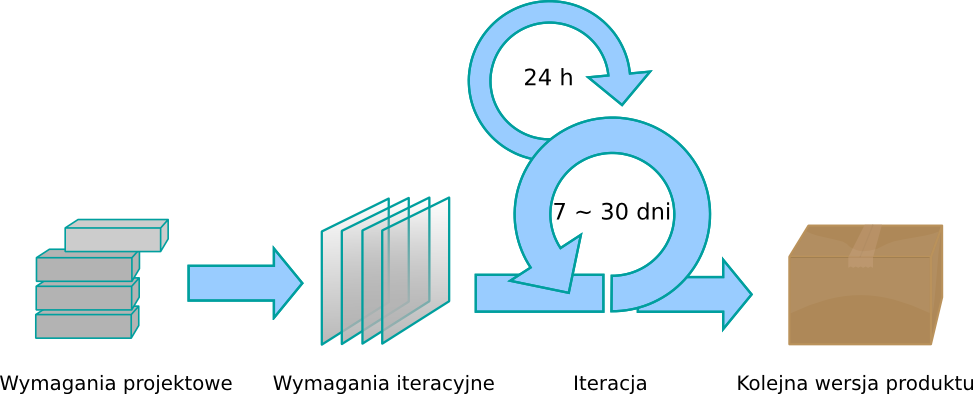
\includegraphics[width=\textwidth]{obrazki/scrum.png}}
\caption[Schemat pracy w metodyce \textit{Scrum}]{Schemat pracy w~kolejnych iteracjach metodyki \textit{Scrum} \cite{scrum.schema}}
\label{fig.rysunek.scrum}
\end{figure}

\subsubsection{Definicje pojęć dla metodyki Scrum} \label{scrum.definicje}

\textit{Iteracją} nazywa się cykl w~procesie wytwarzania oprogramowania, który zostaje zamknięty poprzez zrealizowanie pewnego celu (Rys. \ref{fig.rysunek.scrum}).


Zadania przydzielone zespołowi projektowemu określa się mianem \textit{ticketu}. \textit{Ticket} (z~ang. bilet) określa, jakie obowiązki zostały narzucone na~poszczególnych deweloperów. Jest zwykle odzwierciedleniem żądań i~zaleceń od~klienta.


Główne role, jakie można wymienić w~zespole \textit{Scrum} to:

\begin{enumerate}
  \item \textit{Zespół programistyczny} (ang. \textit{Team}) -- wykonawcy projektu, deweloperzy w~liczbie do~dziewięciu osób. Do ich obowiązków należy ocena trudności zadań (\textit{ticketów}) realizujących założenia projektowe, realizacja tych zadań oraz~zgłaszanie błędów, trudności zaistniałych w~projekcie.
  \item \textit{Właściciel projektu} (ang. \textit{Product Owner}) -- jest to~osoba, firma, grupa~będąca zleceniodawcą (klientem) zatrudniającym zespół programistyczny do~zrealizowania projektu. Zasadniczą rolą właściciela projektu jest przedstawianie założeń, wymagań dotyczących~projektu, rewizja wykonanych zadań tegoż zespołu oraz~konsultowanie zmian. Gdy właścicielem projektu jest jakaś większa jednostka (firma, spółka, grupa), wtedy wyznaczany jest reprezentant odpowiedzialny za~wyżej wymienione czynności.
  \item \textit{Mistrz młyna} (ang. \textit{Scrum Master}) -- osoba odpowiedzialna za~komunikację pomiędzy zespołem programistycznym a~właścicielem projektu. Do~jej obowiązków należy przede wszystkim: ustalanie \textit{sprint meeting'ów}, zgłaszanie intencji zespołu programistycznego, wysyłanie powiadomień o~zmianach w~założeniach.
\end{enumerate}

\subsubsection{Rozpoczęcie pracy w~Scrum} \label{scrum.poczatki}

Zanim zostanie rozpoczęta pierwsza iteracja (\textit{sprint}) należy dokładnie przemyśleć i~omówić możliwości grupy projektowej oraz~skonfrontować je~z~wymaganiami klienta. W~tym celu organizowane jest spotkanie inicjujące pracę nad projektem. Na~takim spotkaniu powinny zostać omówione następujące kwestie:

\begin{enumerate}
  \item \textit{Metody pracy z~klientem} -- klient powinien wiedzieć, jak pracuje zespół, czego może się po~nim spodziewać.
  \item \textit{Założenia projektowe} -- zespół programistyczny dowiaduje się, jakie są~postawione wobec niego oczekiwania.
  \item \textit{Rewizja założeń projektowych} -- zespół programistyczny ma~szansę wypowiedzieć się na~temat kolejnych założeń i~związanych z~nimi trudności.
  \item \textit{Wycena projektu} oraz~ustalenie licencji jego użytkowania.
\end{enumerate}

Po~omówieniu tych zagadnień klient może zdecydować, czy taki sposób pracy mu~odpowiada. W~tym momencie jest w~stanie oszacować, jak długo będzie współpracował nad projektem z~tą~grupą projektową, a~co~za~tym idzie -- jaką ilość pieniędzy może przeznaczyć na~poszczególnych etapach tworzenia projektu.

\subsubsection{Sprint meeting} \label{scrum.sprintmeeting}

\textit{Sprint meeting} zamyka jedną iterację i~rozpoczyna następną. Podczas \textit{sprint meeting'u} realizowane są~następujące działania: sprawdzenie poprawności wykonanych zadań z~poprzedniej iteracji oraz przedyskutowanie planu pracy w następnej iteracji. Pozwala to~klientowi na~pełną kontrolę nad procesem wytwarzania projektu. Do~najważniejszych kwestii omawianych na~\textit{sprint meeting'u} należą:

\begin{enumerate}
  \item \textit{Sprawdzenie stanu wykonanych zadań} -- jeśli zadania zostały dostarczone klientowi jako wykonane, to~klient może je~zweryfikować pod względem ich poprawności. Każde takie zadanie może zostać zaakceptowane (wtedy oznaczone zostaje jako wykonane) bądź nie. Zadanie odrzucone wymaga poprawki -- klient może zdecydować, co~powinno być w~tej sytuacji wykonane. Jeżeli klient ma~wystarczająco funduszy na~wykonanie poprawek, może zlecić poprawkę, jeśli nie, to~zadanie może zostać ,,zamrożone'' i~czekać na~pieniądze potrzebne do~jego realizacji. Oczywiście klient może także zaniechać realizacji zadania.
  \item \textit{Określenie wymagań projektowych} -- klient wymienia swoje oczekiwania względem projektu. Wymagania te~zostają skonfrontowane z~możliwościami zespołu programistycznego (,,tego nie da~się zrobić'', ,,to~jest za~trudne'', ,,to~wymaga lepszego sprzętu'', ,,realizacja tego zadania zajmie \ldots'', ,,koszta tego zadania wyniosą około \ldots'', albo: ,,to~jest proste'', ,,znamy się na~tym''). Zwykle zaistniałe trudności w~realizacji zadań kończą się kompromisem. Po~określeniu możliwości realizacji wymagań tworzone są~zadania.
  \item \textit{Określenie zadań dla grupy projektowej} -- po~,,wycenie'' możliwości deweloperów względem wymagań tworzone są~zadania. Zwykle rozbija się je~na~prostsze, wymagające mniej czasu (według zasady ,,dziel i~zdobywaj'') -- uzyskuje się wtedy płynność w~realizacji zadań, a~praca nad konkretnym wymaganiem podzielona jest pomiędzy członków zespołu.
  \item \textit{Przydzielenie zadań} -- klient po~określeniu i~sprecyzowaniu zadań określa ich priorytet. Niektóre zadania są~ważniejsze -- te~oznaczane są~jako zadania przypisane nadchodzącej iteracji -- nad tymi zadaniami grupa projektowa będzie w~najbliższym czasie pracować. Zadania te~zostają następnie wybierane przez konkretnych deweloperów jako te, które będą przez nich realizowane. Jeżeli po~zakończonej iteracji zostaną zadania niewykonane, to oznacza to, że~grupa nie nadąża z~tempem pracy narzuconym przez klienta.
  \item \textit{Ustalenie ,,dostępności'' deweloperów w~najbliższej iteracji} -- członkowie zespołu mogą z~różnych powodów nie móc pracować w~pewnym okresie czasu. Z~tego względu pod koniec \textit{sprint meeting'u} należy ustalić ile godzin pracy każdy deweloper może przeznaczyć na~najbliższą iterację. Pozwala to~określić ,,siłę'' zespołu oraz~długość iteracji. W~szczególnych przypadkach iteracje mogą zostać przeniesione bądź zawieszone ,,do~odwołania''.
\end{enumerate}

\subsection{Narzędzia Scrum} \label{scrum.narzedzia}

Narzędzi, które wspomagają pracę w~metodyce Scrum jest wiele. Przykładem mogą być tzw. \textit{Issue Tracker'y} -- środowiska do~zarządzania ticketami. Dobrym przykładem takiego \textit{Issue Trackera} jest \textit{PivotalTracker} \cite{pivotaltracker}. Pozwala on~na~kontrolowanie zadań poprzez oznaczanie ich jako wykonanych, bieżących. Przykładowe zastosowanie tego narzędzia w~pracy nad projektem przedstawia rysunek \ref{fig.rysunek.pivotal}.

\begin{figure}[!t]
\centering
\fbox{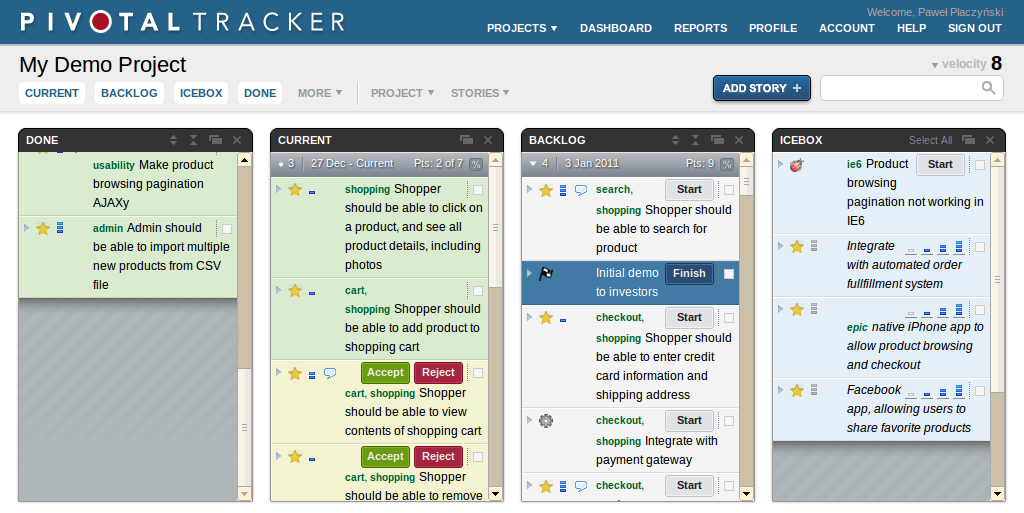
\includegraphics[width=\textwidth]{obrazki/pivotal.png}}
\caption[Narzędzie \textit{PivotalTracker}]{Zastosowanie narzędzia \textit{PivotalTracker} w~pracy nad projektem \cite{pivotaltracker}}
\label{fig.rysunek.pivotal}
\end{figure}

Innym przykładem narzędzia wspomagającego pracę w~projekcie \textit{Scrum} są~testy jednostkowe i~funkcjonalne aplikacji (rozdział \ref{dokumentacja.testy}). Służą one tutaj przede wszystkim rewizji zaimplementowanej funkcjonalności a zatem sprawdzeniu poprawności wykonania zadania. Testy takie są~zatem udokumentowaniem wykonanej pracy przez dewelopera.
